% *****************************************
% UC San Diego PhD thesis template, 2019
% Paolo Gutierrez Gabriel
% Main 
%******************************************

\documentclass{ucsd}
\usepackage{graphicx}
\usepackage{standalone}
\usepackage{chapterbib}


\usepackage{amsmath,amssymb,amsthm} % AMS Math
\usepackage{epsf,epsfig,psfrag} % fig packages
\usepackage{enumitem} % Labels and spacing of itemize & enumerate
\usepackage{makecell} % Fixed width columns for tables
\usepackage{mathptmx} % Times font and math font
\usepackage{cite}   % Dash consecutive citations
\usepackage{framed} % Frame theorems
\usepackage{appendix} % Appendices as subsections
%\usepackage{showframe} % Shows page boundaries
\usepackage[hidelinks]{hyperref} % Links within PDF file


% ---------------------------
% Document contets
% ---------------------------
\begin{document}

%-------------------------------
% Author information:
\title{This is a tribute}
\author{A. Student}
\degreeyear{2019}
\degree{Doctor of Philosophy} 
\field{Department \\
(Sub-track)}
\chair{Professor Chair}

% Committee information (must be alphabetical):
\othermembers{
Professor A \\
Professor B \\ 
Professor C \\
Professor D \\
Professor E
}
\numberofmembers{6} 

%------------------------------------
% Creates title, copyright, and signature pages.
\begin{frontmatter}
\makefrontmatter 

%------------------------------------
% Epigraph page:
\begin{epigraph}
  	% example
\emph{This is the quote I want to print.}\\
Author, "Source"


\end{epigraph}

% Creates TOC, list of figures, and list of tables
% Remember to use \caption[short text]{long text}, and to limit short text to 4 lines.
\tableofcontents
\listoffigures
\listoftables

%------------------------------------
% Acknowledgements - if using published works, must acknowledge here
\begin{acknowledgements} 
		First and foremost, I would like to thank my advisor for their guidance, support, and inspiration.
	%
	I would also like to thank my family
	%
	The chapters of this dissertation consist of published and submitted journal articles.
	The dissertation author was either the primary or secondary investigator and author of each of these papers.
	%
\begin{itemize}
	% Chapter 1

	% Chapter 2
	\item Chapter 2, in full, is a reprint of the material as it appears in """"
	%
	The dissertation author was the primary investigator and author of this paper. 

	% Chapter 3
	\item Chapter 3, in part, is a reprint of materials as they appear in [N] papers. First is Alasfour et al., JNE 2019. Second is Chen et al., JTEHM 2018. 
	%
	The dissertation author was the secondary investigator and author of both of these papers. 

	% Chapter 4
	\item Chapter 4, in full, is a reprint of the material as it appears in """" 
	%
	The dissertation author was the primary investigator and author of this paper.

	% Chapter 5
	\item Chapter 5, in part, is currently being prepared for submission for publication of the material.  
	%
	The dissertation author was the primary investigator and author of this material.
	%
\end{itemize}	
\end{acknowledgements}

%------------------------------------
% Vita 
%(be consistent with abbreviations (B.S. and M.S. or Bachelor of Science and Master of Science)
\begin{vitapage}
	% Vita
	\begin{vita}
	% CV must be included colleges attended and degrees earned; 
% professional appointments optional;
% publications optional 
  \item[2013] Bachelor of Science in Engineering Physics,
  		Stanford University, Stanford 
  \item[2013 -- 2019] Graduate Student Researcher,
  		University of California, San Diego
  \item[2015] Master of Science in Electrical Engineering
  		(Medical Devices \& Systems),
  		University of California, San Diego
  \item[2019] Doctor of Philosophy in Electrical Engineering
  		(Medical Devices \& Systems),
  		University of California, San Diego 
	\end{vita}

	% Publications
	\begin{publications}
	% currently running chicago style. Choose one that lists ALL authors (no et al.)
\item This is a paper I published

\item This is another one
	\end{publications}
\end{vitapage}

%------------------------------------
% Abstract
\begin{abstract}
% abstract text only
\par\indent
	This is the text that represents the abstract of my thesis. It will describe everything from the conceptual model motivating why we study motor behaviors and the brain as a control unit. It will also describe how task-based studies do this and compare it against my approach. It will discuss, broadly, how my approaches address specific needs in this problem. It will specify the results / demonstrations / methods being reported in the thesis. 
\end{abstract}
\end{frontmatter}


% Main text
% https://tex.stackexchange.com/questions/34786/why-are-my-include-files-ignored
%===========================================

% *****************************************
% {thesis template}
% Author
% Introduction chapter
%******************************************

%-----------

% \vspace{6em}
\chapter{Introduction}

This topic is important and here is why...

\section{Background}~ Background information. Example citations include this paper\cite{miller2014broadband} and these papers speech\cite{wilson1999spike, scheuer2004data, furbass2015prospective}.


\section{Challenges}~ 

\section{Proposed method}~ 

% Chapter Bibliography references MASTER bibliography
\clearpage
\bibliographystyle{unsrt}
\bibliography{bib}

% Repeat acknowledgements here


% *****************************************
% {thesis template}
% Author
% Introduction chapter
%******************************************

\chapter{Title of chapter 2}

% ---------------------------------------------------------------------------
% Use an abstract to explain copy/paste papers below... the theme

  \begin{center}
  \textbf{\LARGE Abstract}
  \end{center}

  This chapter considers SOMETHING.
  %
  We show that...

\clearpage

% ---------------------------------------------------------------------------
\section{Introduction} 

In this chapter, we focus on SOMETHING

%-----------------------------------------------
\subsection{Network Model}
%-----------------------------------------------


In addition,~\cite{alasfour2018coarse} demonstrates that from such data, behavior-specific contexts can be discriminated from freely recorded neural activity.

Here is a figure:
\begin{figure}[!ht]
\centering
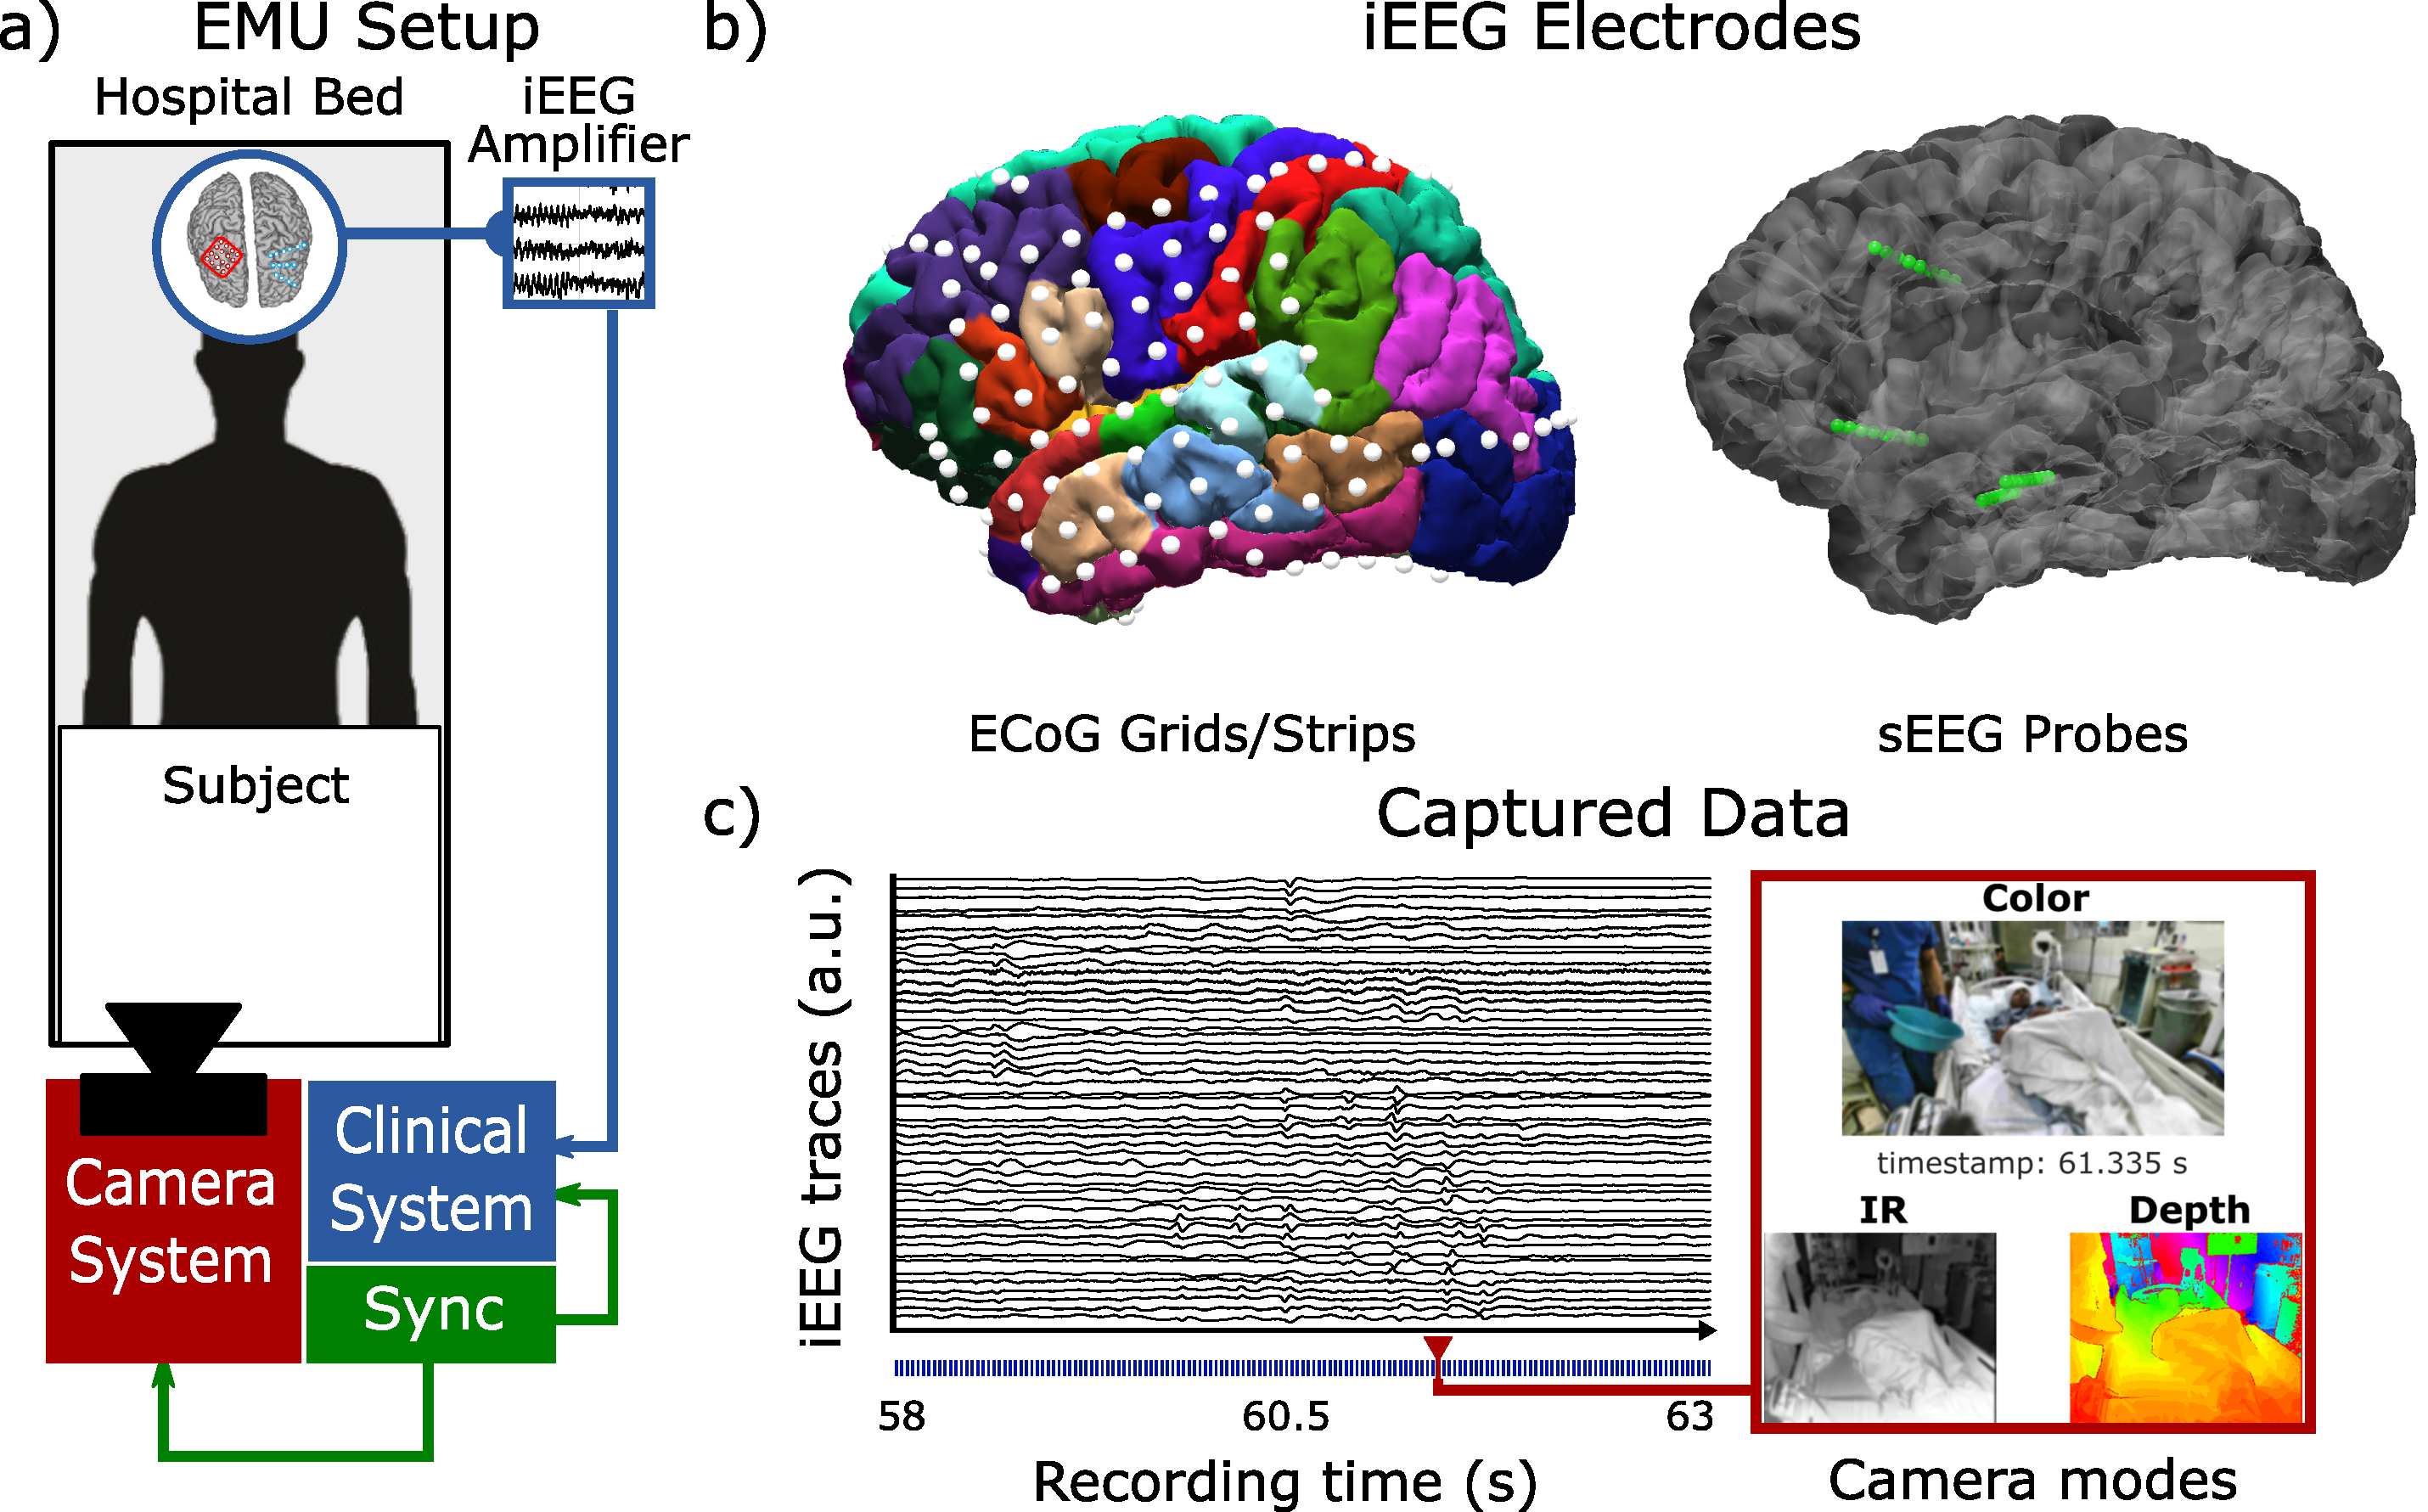
\includegraphics[width=0.85\textwidth]{img/method_setup.pdf}
\caption[This is the short form of the caption. It has to be no more than 4 lines.]{\textbf{Diagram of experimental setup for recording behavioral video simultaneously with intracortical activity (ECoG, sEEG) from subjects in the epilepsy monitoring unit.} \textbf{a)} The experimental setup places the video recording system at the foot of the hospital bed facing the subject to capture the subject and their immediate surroundings. \textbf{b)} A typical subject has over 100 electrodes placed according to clinical need, as shown in the reconstructed coverage of ECoG and sEEG for Subject 1. A combination of subdural grid and strip electrodes (ECoG) covers many regions of the cortical surface, depicted by the Desikan-Killiany parcellation~\cite{desikan2006automated}, while stereotactic depth probes (sEEG) sample deep and superficial brain structures. \textbf{c)} During the study, videos (blue) of the subject moving in an uninstructed and unstructured manner are captured using a Kinect for Windows (v2) sensor. An example of the sensor modalities is framed in red. A subset of 50 neural traces recorded in parallel shown underneath, aligned $\leq 5ms$ of each video frame. Data collected in this manner captures an external and intracortical representation of each subject's movement. A preliminary demonstration using neural features in relation to movement segments marked using only the color video stream is detailed in this work.}
\label{fig-setup}
\end{figure}

%-------------------------------------
\subsection{Related Work} 
%-------------------------------------
Text

%------------------------------------------
\subsection{Our Contributions}
%------------------------------------------
Text

\clearpage

%-------------------------------------------------------

%------------------------------------------------
\section{Open Questions}
\label{ch2:questions}

% % Chapter Bibliography
\clearpage
\bibliographystyle{unsrt}
\bibliography{bib}

% Repeat acknowledgements here


% *****************************************
% {thesis template}
% Author
% Introduction chapter
%******************************************

\chapter{Title of chapter 3}

% ---------------------------------------------------------------------------
% Use an abstract to explain copy/paste papers below... the theme

  \begin{center}
  \textbf{\LARGE Abstract}
  \end{center}

  This chapter considers SOMETHING.
  %
  We show that...

\clearpage

% ---------------------------------------------------------------------------
\section{Introduction} 

In this chapter, we focus on SOMETHING

%-----------------------------------------------
\subsection{Network Model}
%-----------------------------------------------


Here's a new citation that no previous chapter includes ~\cite{akaike2011akaike}

This is a table: Note that you are reponsible for adjusting table format to fit thesis format.
\begin{table}
\caption[This is the short table caption that must be 4 lines MAX.]{This is the long table caption.} 
% \begin{indented}
\begin{center}
% \lineup
% \item[]
\begin{tabular}{@{}*{7}{c}}
\br                              
Subject No. & Patient ID & Recording dur. (hrs.) & Implant type & Coverage & Handedness & Age (y.o.)/Sex\cr 
\mr
1 & NY531 & 2.25 & ECoG/sEEG & LHem. & R & 48/M \\ \cr
%NY596 & 48 & ECoG & RHem. & R\\ \cr
2 & RCH1 & 9 & sEEG & L FL/TL & R & 18/F \\ \cr
3 & RCH3 & 24 & sEEG & L/R FL/TL & R & 17/M \\ 
\br
\end{tabular}
% \end{indented}
\end{center}
\end{table}



%-------------------------------------
\subsection{Related Work} 
%-------------------------------------
Text

%------------------------------------------
\subsection{Our Contributions}
%------------------------------------------
Text

\clearpage

%-------------------------------------------------------

%------------------------------------------------
\section{Open Questions}
\label{ch2:questions}

% % Chapter Bibliography
\clearpage
\bibliographystyle{unsrt}
\bibliography{bib}

% Repeat acknowledgements here




% \chapter{Parameterization of Unstructured Movement Sequences}\label{ch:kinematics}
% % \input{cap-src/cap.tex}

% \chapter{Big Picture Discussion}\label{ch:discussion}
% \input{disc.tex}


\end{document}
